
\chapter{Theory}

\section{Standard model}

Standard model(SM) describes the properties of the fundamental particles currently known in the universe and the interactions amount them.  The discovery of Higgs boson in 2012 implement the last missing piece in SM.  The particles in SM is shown in Figure.~\ref{fig:SM_particles}. Besides Higgs boson, there are three generations of leptons and quarks and four gauge bosons. 
Leptons and quarks are fermions that compose the matters currently known in the universe, while the gauge bosons serve as the mediators of interactions.  

SM is a gauge theory, which describes three natural force, the strong, electromagnetic and weak force by symmetry group $SU(3)_{C}\times SU(2)_{L}\times U(1)_{Y}$. Electroweak section is described by $SU(2)_{L}\times U(1)_{Y}$. The L in $SU(2)_{L}$ stands for the left chiral signature of the weak interaction and the Y in $U(1)_{Y}$ stands for the weak hypercharge. Strong interaction is described by $SU(3)_{C}$, in which the C stands for the colors of quarks.  Photons, gluons and $W^{\pm}$, Z bosons are the mediators of electromagnetic, strong and weak force respectively.  Gravity force is not included in SM. Each particles in Figure.~\ref{fig:SM_particles} has its anti-particle or the anti-particle is the particle itself. The force and mediators characters are summarized in Table.~\ref{Mediator_infor}

\begin{figure}[htbp] 
\centering
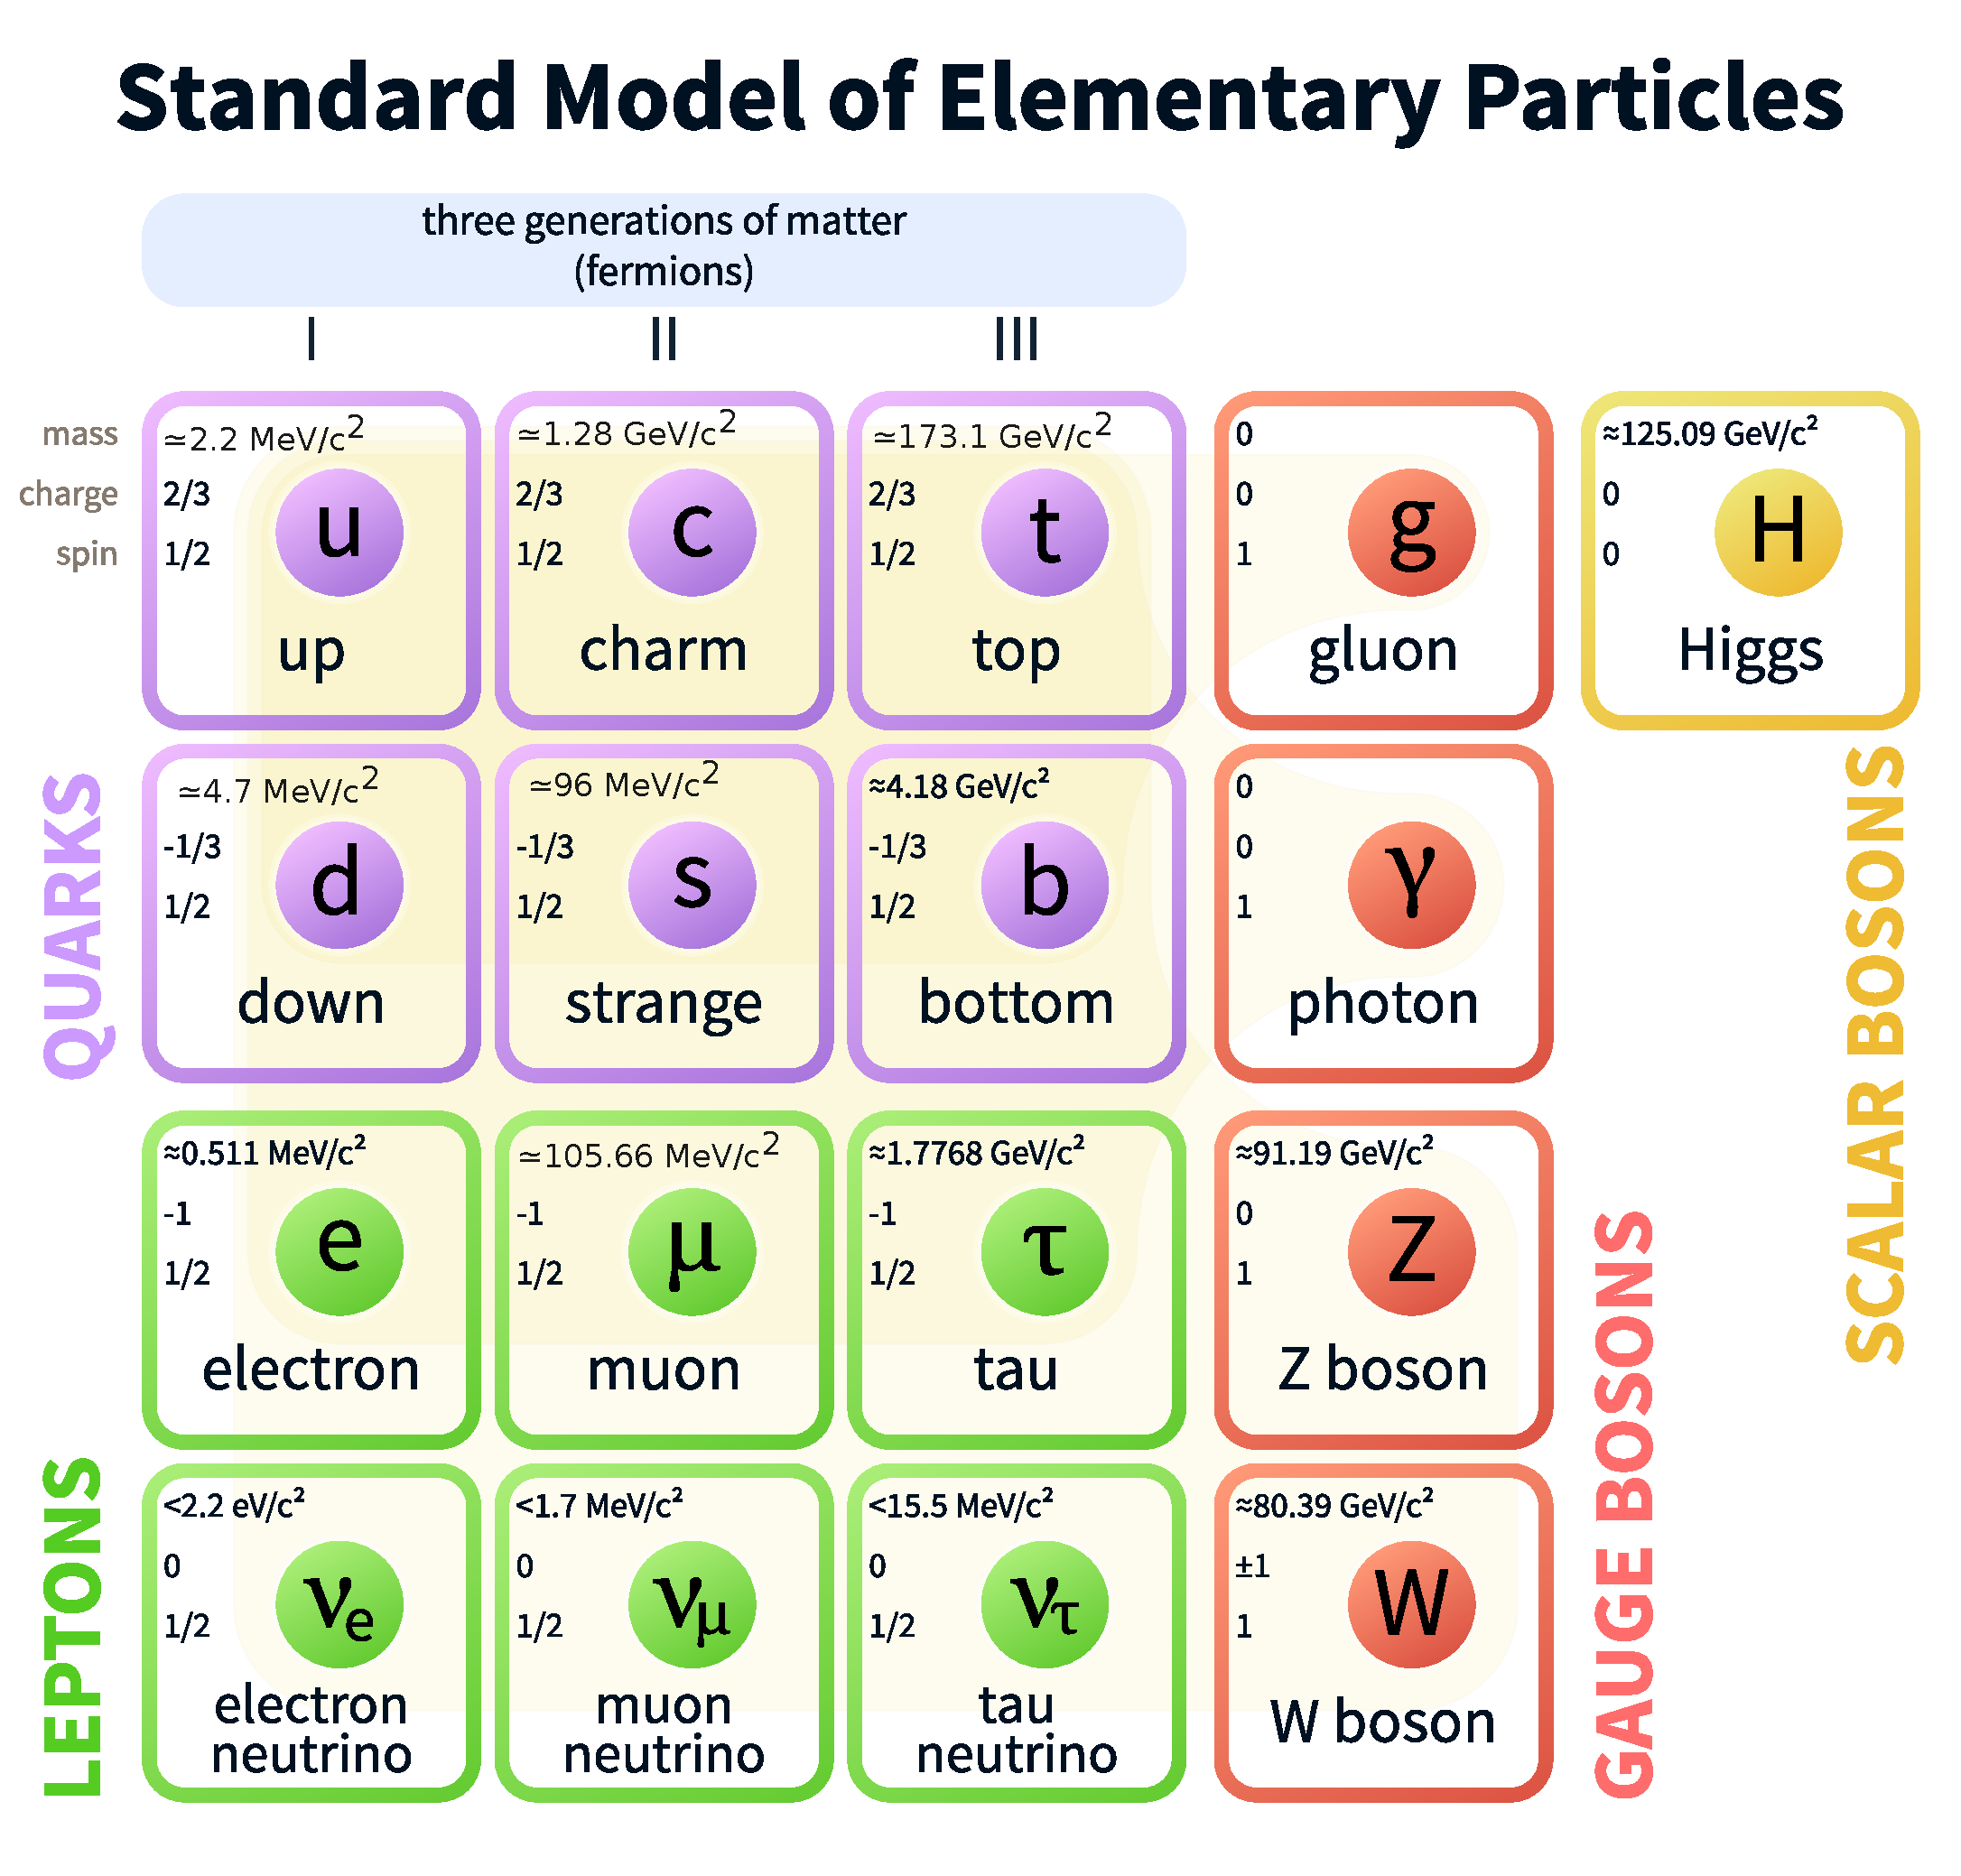
\includegraphics[width=0.8\textwidth]{chapter2/SM_particle_table.pdf}
\caption{Standard model particle group\cite{SM_particletable}}
\label{fig:SM_particles}
\end{figure}


\begin{table}[htp]
\caption{Mediators in standard model~\cite{Griffiths:111880}}
\begin{center}
\begin{tabular}{|c|c|c|c|c|}
\hline
Force & Mediator & Charge & Mass(GeV) & Range(m)   \\\hline
Strong                & g(8 gluons)                  & 0 & 0 & $10^{-15}$   \\\hline
Electromagnetic & $\gamma$(photon)     & 0 & 0 &   $\infty$   \\\hline
Weak                  &  $W^{\pm}$                &$\pm$1 & 80.379 &$10^{-18}$\\
                           & Z                                &  0         & 91.1876 &  $10^{-18}$ \\\hline
\end{tabular}
\end{center}
\label{Mediator_infor}
\end{table}%


Fermion fields in SM can be further categorized. In weak interaction, left-handed fermions are isodoublets, while right-handed fermions are isosinglets. Only the left-handed fermions or right-handed anti-fermions participate in the weak interaction. Weak hypercharge is a combined quantity, which is defined by the electric charge Q the third component of the weak isospin $I^{3}_{f}$, $Y=Q-I^{3}_{f}$. Weak interaction, together with Electromagnetic interaction are best described and understood by the electro-weak theory, which is be further discussed in the next section.  Quarks are described by SU(3), which are color triplets, while leptons are color singlets.   

Mediators in the interaction are represented by the gauge boson fields. $B_{\mu}$ is associated with symmetry $U(1)_{Y}$ and the corresponds generator is Y. $W_{\mu}^{1,2,3}$ are associated to $SU(2)_{L}$ symmetry with the generator $T^{a}$(a=1,2,3). $T^{a}$ are the $2\times2$ Pauli matrices. $G_{\mu}^{1...,8}$ are associated with the $SU(3)_{c}$ symmetry and the corresponding generators are the Gell-Mann matrices.  The field strengths is expressed as 






The masses of the gauge bosons in weak interaction and fermions are generated by spontaneous symmetry breaking. Fermions specifically are generated by Higgs mechanism.  If mass terms are directly added in, the local $SU(2)\times U(1)$ will be destroyed~\cite{DJOUADI20081}. Local symmetry referring to the transformations on the fields are the functions that involve space-time.  






\subsection{spontaneous symmetry breaking}



\subsection{Higgs mechanism}




\section{Lepton flavour violation in beyond stand model theories}


Three questions need to answer:
1. Higgs in standard model
2. Why LFV is not possible in SM
3. LFV in beyond standard models

why LFV is not possible in SM